\frame{
	\frametitle{0G}
	\begin{columns}
		\begin{column}{0.5\textwidth}
      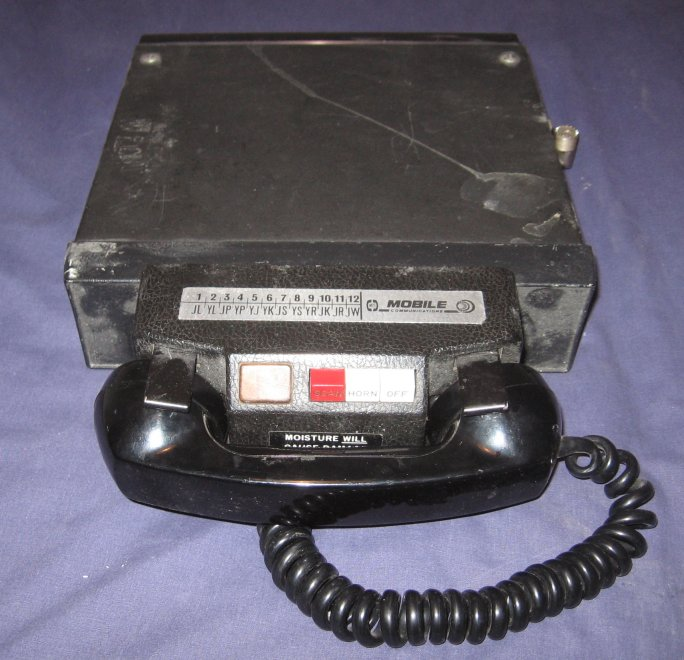
\includegraphics[height=6cm]{pictures/mobile_radio_telephone}
    \end{column}
    \hfill
    \begin{column}{0.5\textwidth}
      \begin{itemize}
        \item First mobile systems with access to public network
        \item Most of them needed human operators, had local area code and no cell switching % most of them were in a trunk
        \item 1952: A-Netz in West Germany % equal to MTS (USA), 11.000 users at the peak, the limit
        \item Other systems in the USSR, Norway, Finland and the UK
        \item 1972: B-Netz in West Germany % equal to IMTS (USA), no human operators needed, 27.000 users at the peak, the limit
      \end{itemize}
    \end{column}
  \end{columns}
}
